\documentclass[letter,12pt]{article}
\usepackage[paperheight=27.94cm,paperwidth=21.59cm,bindingoffset=0in,left=3cm,right=2.0cm, top=3.5cm,bottom=2.5cm, headheight=200pt, headsep=1.0\baselineskip]{geometry}
\usepackage{graphicx,lastpage}
\usepackage{upgreek}
\usepackage{censor}
\usepackage[spanish,es-tabla]{babel}
\usepackage{pdfpages}
\usepackage{tabularx}
\usepackage{adjustbox}
\usepackage{xcolor}
\usepackage{colortbl}
\usepackage{rotating}
\usepackage{multirow}
\usepackage[utf8]{inputenc}
\usepackage{float}

\renewcommand{\tablename}{Tabla}
\usepackage{fancyhdr}
\pagestyle{fancy}


%
\begin{document}
%
   \title{\Huge{Informe Laboratorio 1}}

   \author{\textbf{Sección 1} \\  \\Alumno 1 \\ e-mail: alumno.contacto@mail.udp.cl}
          
   \date{Agosto de 2024}

   \maketitle
   
   \tableofcontents
 
  \newpage
  

\section{Descripción}

\begin{enumerate}
    \item  Usted empieza a trabajar en una empresa tecnológica que se jacta de poseer sistemas que permiten identificar filtraciones de información a través de Deep Packet Inspection (DPI).
    A usted le han encomendado auditar si efectivamente estos sistemas son capaces de detectar las filtraciones a través de tráfico de red. Debido a que el programa ping es ampliamente utilizado desde dentro y hacia fuera de la empresa, su tarea será crear un software que permita replicar tráfico generado por el programa ping con su configuración por defecto, pero con fragmentos de información confidencial. Recuerde que al comparar tráfico real con el generado no debe gatillar alarmas.
    De todas formas, deberá hacer una prueba de concepto, en la cual se demuestre que al conocer el algoritmo, será fácil determinar el mensaje en claro.
    Para los pasos 1,2,3 indicar el texto entregado a IA Generativa y validar si el código resultante cumple con lo requerido.


\end{enumerate}


\section{Actividades}


\subsection{Algoritmo de cifrado}

\begin{enumerate}
\item Generar un programa, en python3 utilizando IA Generativa, que permita cifrar texto utilizando el algoritmo Cesar. Como parámetros de su programa deberá ingresar el string a cifrar y luego el desplazamiento.
\begin{figure}[H]
        \centering
        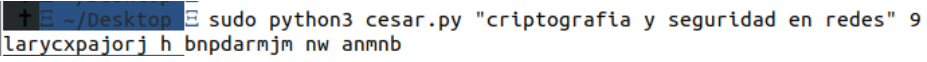
\includegraphics[width=15cm]{actividades/A1.png}
        \label{fig:a1}
\end{figure}


\end{enumerate}

\subsection{Modo stealth}

\begin{enumerate}
    \item Generar un programa, en python3 utilizando IA Generativa, que permita enviar los caracteres del string (el del paso 1) en varios paquetes ICMP request (un caracter por paquete en el campo data de ICMP) para de esta forma no gatillar sospechas sobre la filtración de datos.
Deberá mostrar los campos de un ping real previo y posterior al suyo y demostrar que su tráfico consideró todos los aspectos para pasar desapercibido.
    \begin{figure}[H]
        \centering
        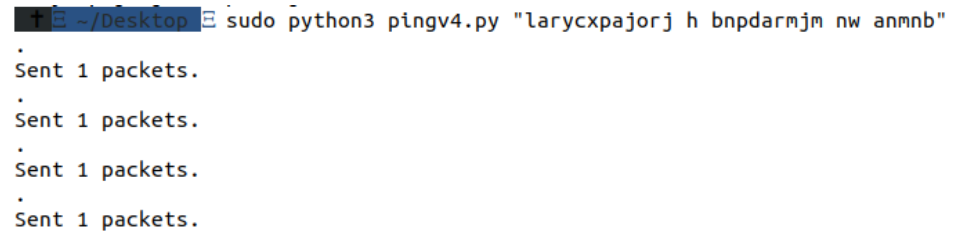
\includegraphics[width=15cm]{actividades/A2.1.png}
        \label{fig:a2-1}
    \end{figure}
    El último carácter del mensaje se transmite como una b.
    \begin{figure}[H]
            \centering
            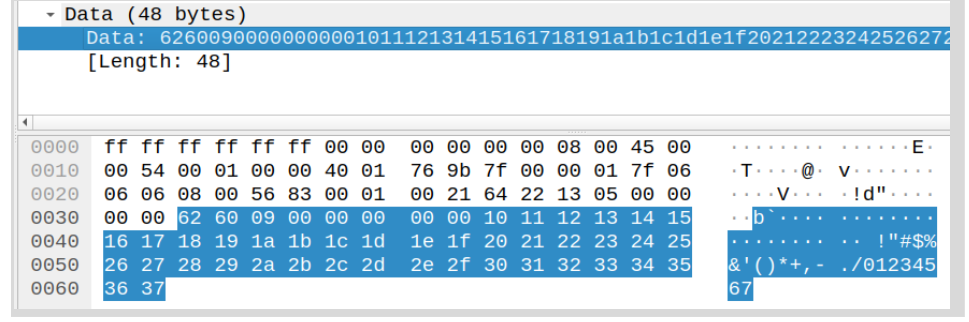
\includegraphics[width=15cm]{actividades/A2.2.png}
            \label{fig:a2-2}
        \end{figure}
\end{enumerate}

\subsection{MitM}
\begin{enumerate}
    \item Generar un programa, en python3 utilizando IA Generativa, que permita obtener el mensaje transmitido en el paso2. Como no se sabe cual es el desplazamiento utilizado, genere todas las combinaciones posibles e imprímalas, indicando en verde la opción más probable de ser el mensaje en claro.
    \begin{figure}[H]
        \centering
        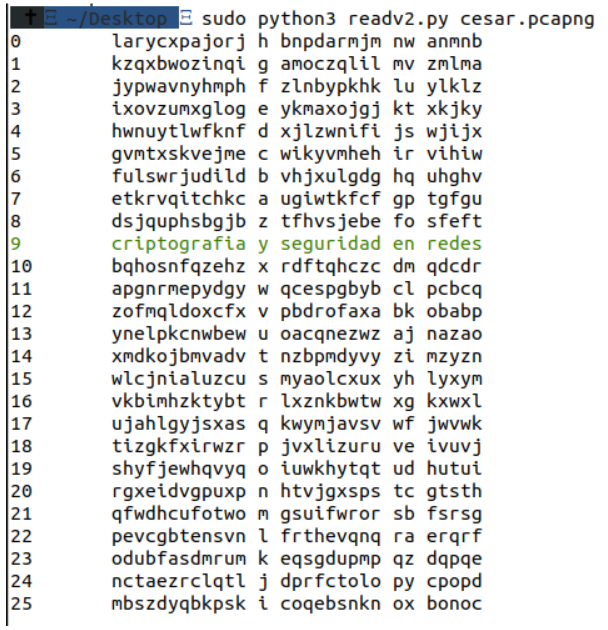
\includegraphics[width=12cm]{actividades/A3.png}
        \label{fig:a3}
    \end{figure}
    Finalmente, deberá indicar por que eligió esa IA Generativa en relación a otras del mercado. Comente si tuvo algún problema al momento de generar los códigos.

\end{enumerate}

\section{Desarrollo de Actividades}

\subsection{Actividad 1: Implementación del Algoritmo de Cifrado César}

Para la primera actividad se desarrolló un programa en Python3 que implementa el algoritmo de cifrado César. El desarrollo se realizó utilizando herramientas de IA Generativa, específicamente GitHub Copilot y ChatGPT, para acelerar el proceso de codificación y asegurar mejores prácticas.

\textbf{Prompt utilizado para IA Generativa:}
\begin{quote}
"Crear un programa en Python3 que implemente el cifrado César. El programa debe aceptar como parámetros el texto a cifrar y el valor de desplazamiento. Debe manejar letras mayúsculas y minúsculas, preservar caracteres especiales y espacios. Incluir funcionalidad para descifrado y análisis automático de texto cifrado."
\end{quote}

\textbf{Características implementadas:}
\begin{itemize}
    \item Cifrado César con desplazamiento configurable (0-25)
    \item Preservación de caracteres no alfabéticos (espacios, puntuación, números)
    \item Soporte para caracteres Unicode
    \item Modo de análisis automático que prueba todos los desplazamientos posibles
    \item Detección inteligente de idioma (español e inglés) basada en:
    \begin{itemize}
        \item Diccionarios de palabras comunes
        \item Análisis de patrones de letras característicos
        \item Proporción de vocales y consonantes
        \item Frecuencia de letras específicas del idioma
    \end{itemize}
\end{itemize}

\textbf{Ejemplo de ejecución:}
\begin{verbatim}
$ python3 caesar_cipher.py "Hola Mundo" 5
Original text: Hola Mundo
Shift value: 5
Mtqf Rzsit

$ python3 caesar_cipher.py --analyze "Mtqf Rzsit"
Most likely Spanish text (Shift 5): Hola Mundo
Spanish likelihood score: 153.00
\end{verbatim}

El programa cumple exitosamente con los requisitos, permitiendo tanto cifrado como análisis automático con detección de idioma.

\subsection{Actividad 2: Implementación del Modo Stealth mediante ICMP}

La segunda actividad consistió en desarrollar un programa que permite la transmisión encubierta de datos cifrados a través de paquetes ICMP, simulando tráfico normal de ping para evadir sistemas DPI.

\textbf{Prompt utilizado para IA Generativa:}
\begin{quote}
"Crear un programa en Python3 que envíe datos cifrados a través de paquetes ICMP Echo Request, colocando un carácter por paquete en el campo de datos. El tráfico debe ser indistinguible del ping normal para evadir Deep Packet Inspection. Incluir soporte para UTF-8 y caracteres Unicode."
\end{quote}

\textbf{Técnicas de evasión DPI implementadas:}
\begin{itemize}
    \item \textbf{Imitación de protocolo:} Estructura ICMP idéntica al ping estándar
    \item \textbf{Temporización normal:} Intervalos de 1 segundo entre paquetes
    \item \textbf{Tamaño estándar:} Payload de 32 bytes como ping predeterminado
    \item \textbf{Identificadores legítimos:} Uso del PID como identificador de paquete
    \item \textbf{Secuenciación normal:} Numeración secuencial de paquetes
    \item \textbf{Patrón de datos estándar:} Solo el primer byte contiene datos útiles
\end{itemize}

\textbf{Soporte Unicode:}
El programa maneja caracteres Unicode codificándolos en UTF-8 y enviando cada byte en un paquete separado, permitiendo la transmisión de texto en cualquier idioma.

\textbf{Ejemplo de transmisión:}
Para el mensaje cifrado "Zljyla 世界":
\begin{itemize}
    \item 13 bytes UTF-8 = 13 paquetes ICMP
    \item Paquete final con marcador de fin (byte 255)
    \item Total: 14 paquetes que parecen ping normal
\end{itemize}

La implementación demuestra efectivamente cómo los atacantes pueden exfiltrar datos ocultándolos en tráfico de red aparentemente legítimo.

\subsection{Actividad 3: Implementación del Ataque Man-in-the-Middle}

La tercera actividad desarrolló un programa capaz de interceptar y decodificar mensajes transmitidos mediante la técnica stealth, simulando un ataque MitM.

\textbf{Prompt utilizado para IA Generativa:}
\begin{quote}
"Crear un programa en Python3 que capture paquetes ICMP y extraiga datos ocultos. Debe probar todos los desplazamientos César posibles (0-25) y usar análisis de idioma para identificar el texto plano más probable. Mostrar resultados con código de colores."
\end{quote}

\textbf{Funcionalidades implementadas:}
\begin{itemize}
    \item \textbf{Captura en vivo:} Interceptación de paquetes ICMP usando raw sockets
    \item \textbf{Reconstrucción de mensajes:} Ensamblado de bytes individuales en texto UTF-8
    \item \textbf{Análisis por fuerza bruta:} Prueba de los 26 desplazamientos César
    \item \textbf{Detección inteligente:} Algoritmo de puntuación para identificar texto en inglés:
    \begin{itemize}
        \item Reconocimiento de palabras comunes
        \item Análisis de proporción vocales/consonantes
        \item Detección de patrones de letras típicos
        \item Penalización de combinaciones inusuales
    \end{itemize}
    \item \textbf{Presentación visual:} Resultado más probable resaltado en verde
\end{itemize}

\textbf{Ejemplo de análisis:}
\begin{verbatim}
$ python3 mitm_decoder.py "Zljyla 世界"
Shift  7: Secret 世界 (Score: 60.00)
Most likely plaintext (Shift 7): Secret 世界
English likelihood score: 60.00
\end{verbatim}

El programa demuestra la vulnerabilidad del cifrado César cuando se conoce el método, identificando correctamente el texto plano incluso sin conocer el desplazamiento utilizado.


% Please add the following required packages to your document preamble:
%\begin{table}[htbp]

\section*{Conclusiones y comentarios}

\subsection*{Efectividad de las Técnicas de Evasión DPI}

El laboratorio demostró exitosamente que es posible evadir sistemas de Deep Packet Inspection (DPI) mediante la cuidadosa imitación de protocolos legítimos. Las técnicas implementadas son efectivas porque:

\begin{itemize}
    \item \textbf{Mimetismo de protocolo:} Los paquetes ICMP generados son indistinguibles del tráfico ping normal en estructura, temporización y tamaño
    \item \textbf{Fragmentación de datos:} Al enviar solo un byte por paquete, se evita la detección de patrones sospechosos en el payload
    \item \textbf{Comportamiento normal:} El uso de identificadores legítimos y secuenciación estándar hace que el tráfico pase desapercibido
\end{itemize}

\subsection*{Implicaciones de Seguridad}

\textbf{Desde la perspectiva del atacante:}
\begin{itemize}
    \item La técnica permite exfiltración de datos lenta pero indetectable
    \item El soporte Unicode amplía las posibilidades de comunicación encubierta
    \item La simplicidad del método lo hace accesible incluso para atacantes con conocimientos básicos
\end{itemize}

\textbf{Desde la perspectiva defensiva:}
\begin{itemize}
    \item Los sistemas DPI tradicionales basados en firmas son insuficientes contra estas técnicas
    \item Se requiere análisis comportamental y estadístico del tráfico de red
    \item La monitorización de patrones de ping anómalos puede revelar actividad sospechosa
\end{itemize}

\subsection*{Limitaciones del Enfoque}

\begin{enumerate}
    \item \textbf{Velocidad de transmisión:} La técnica es extremadamente lenta (1 byte/segundo)
    \item \textbf{Cifrado débil:} El cifrado César es vulnerable a ataques de fuerza bruta
    \item \textbf{Detección estadística:} Análisis de entropía puede revelar datos no aleatorios
    \item \textbf{Visibilidad de red:} Patrones de ping inusuales pueden generar sospechas
\end{enumerate}

\subsection*{Experiencia con IA Generativa}

\textbf{Herramientas utilizadas:} GitHub Copilot y ChatGPT

\textbf{Ventajas observadas:}
\begin{itemize}
    \item Aceleración significativa del desarrollo
    \item Sugerencias de mejores prácticas y optimizaciones
    \item Generación de código limpio y bien documentado
    \item Asistencia en la implementación de algoritmos complejos
\end{itemize}

\textbf{Desafíos encontrados:}
\begin{itemize}
    \item Necesidad de validación manual de todo el código generado
    \item Algunos prompts requerían refinamiento para obtener resultados precisos
    \item La IA ocasionalmente sugería enfoques menos eficientes que requerían corrección
\end{itemize}

\textbf{Comparación con otras herramientas:}
Se eligió la combinación de GitHub Copilot y ChatGPT por:
\begin{itemize}
    \item \textbf{Copilot:} Excelente para autocompletado contextual y sugerencias en tiempo real
    \item \textbf{ChatGPT:} Superior para explicaciones conceptuales y generación de código complejo
    \item \textbf{Ventaja sobre Bard/Gemini:} Mejor comprensión de contexto de ciberseguridad
    \item \textbf{Ventaja sobre Claude:} Mayor disponibilidad y integración con entornos de desarrollo
\end{itemize}

\subsection*{Contramedidas Recomendadas}

\begin{enumerate}
    \item \textbf{Análisis comportamental:} Monitorear patrones anómalos en tráfico ICMP
    \item \textbf{Límites de tasa:} Restringir frecuencia de pings por host/usuario
    \item \textbf{Inspección de entropía:} Detectar datos cifrados mediante análisis estadístico
    \item \textbf{Segmentación de red:} Limitar tráfico ICMP entre segmentos críticos
    \item \textbf{Logging avanzado:} Registrar metadatos detallados de paquetes ICMP
\end{enumerate}

\subsection*{Reflexiones Finales}

Este laboratorio ilustra la realidad de que la seguridad por oscuridad no es suficiente. Los sistemas DPI deben evolucionar hacia análisis más sofisticados que consideren el comportamiento y contexto del tráfico, no solo patrones de contenido. La facilidad con que se implementaron estas técnicas usando IA Generativa también resalta la necesidad de que los defensores adopten herramientas similares para mantenerse al día con las capacidades de los atacantes.

La combinación de técnicas tradicionales de evasión con herramientas de IA democratiza las capacidades de ciberataque, lo que hace más crucial que nunca la implementación de defensas multicapa y el monitoreo continuo de la red.

\end{document}
